\documentclass[hidelinks,12pt,a4paper,openright,twoside]{book}
\usepackage[italian]{babel}
\usepackage[utf8]{inputenc}
\usepackage{fourier}

% Images
\usepackage{graphicx}
\usepackage{caption}
\usepackage{subcaption}
\usepackage{float}
\graphicspath{ {../Images} }

% Stop hyphenation
\usepackage[none]{hyphenat}

% Background page image.
\usepackage{eso-pic}
\usepackage[top=2cm, bottom=2cm, outer=0cm, inner=0cm]{geometry}

% To hide images
\usepackage[allfiguresdraft]{draftfigure}

% To color text parts
\usepackage{xcolor}

% Adjust margins
\usepackage{changepage}

% Minipages in the same line
\usepackage{tabularx}

% License
\usepackage[
type={CC},
modifier={by-nc-sa},
version={4.0},
]{doclicense}

\begin{document}
	
	% Remove page number
	\pagestyle{empty}
	
	% Album Cover
	\begin{center}
		\vspace*{15mm}
		\fboxrule=4pt{
		\fbox{ %                  height                                width
			\begin{minipage}[l] [\dimexpr 0.150\textwidth \relax] [t] {\dimexpr .460\textwidth \relax}
				\vspace{5mm}
				\centering{\large \textbf{Album sulle opere del Museo Civico\\}}
				\bigskip
				Alice Balestieri \\
				Francesco Rombaldoni
			\end{minipage}
			}
		}
	\end{center}
	
	% Background image
	\AddToShipoutPictureBG*{\includegraphics[draft=false, width=\paperwidth,height=\paperheight]{example-image}}
	\newpage
	
	%--------- Page 1 ----------
		
			%  Mengaroni_Ferruccio-Medusa
			\begin{minipage}{0.5\linewidth}
				\begin{center}
					\setdf{content={\textcolor{white}{\hspace{25mm} \Large \#1}}}
					\colorbox{black}{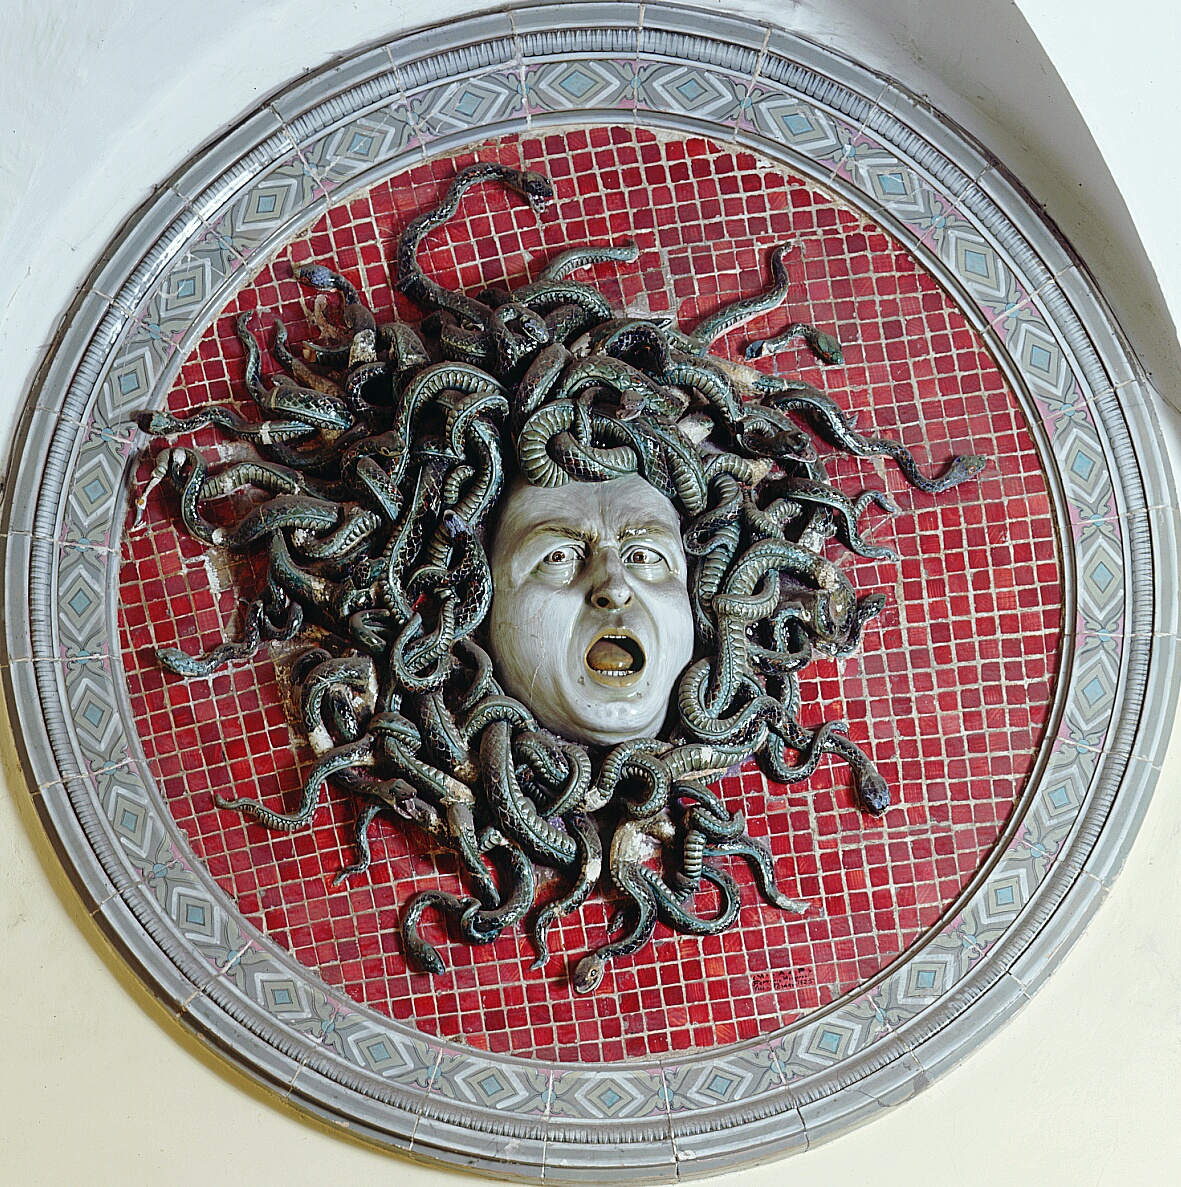
\includegraphics[scale = 1.2]{Mengaroni_Ferruccio-Medusa.jpg}}
				\end{center}
				\begin{center}
					\begin{minipage}{\linewidth}
						\raggedright
						"La Medusa" accoglie i visitatori introducendoli alle sale espositive; si tratta dell'ultima opera di Ferruccio Mengaroni.\\
						L'imponente Medusa ritrae i lineamenti dell'artista pesarese: la leggenda narra che, per riprodurre il proprio volto, egli si fosse servito di uno specchio che poi si ruppe.
					\end{minipage}
			\end{center}
			\end{minipage}
		
		\vspace{10mm}
		
			\begin{adjustwidth}{0mm}{5mm}
				\raggedleft{
				% Bellini_Giovanni-Incoronazione_della_Vergine
				\begin{minipage}{0.5\linewidth}
					\begin{center}
						\setdf{content={\textcolor{white}{\hspace{25mm} \Large \#2}}}
						\colorbox{black}{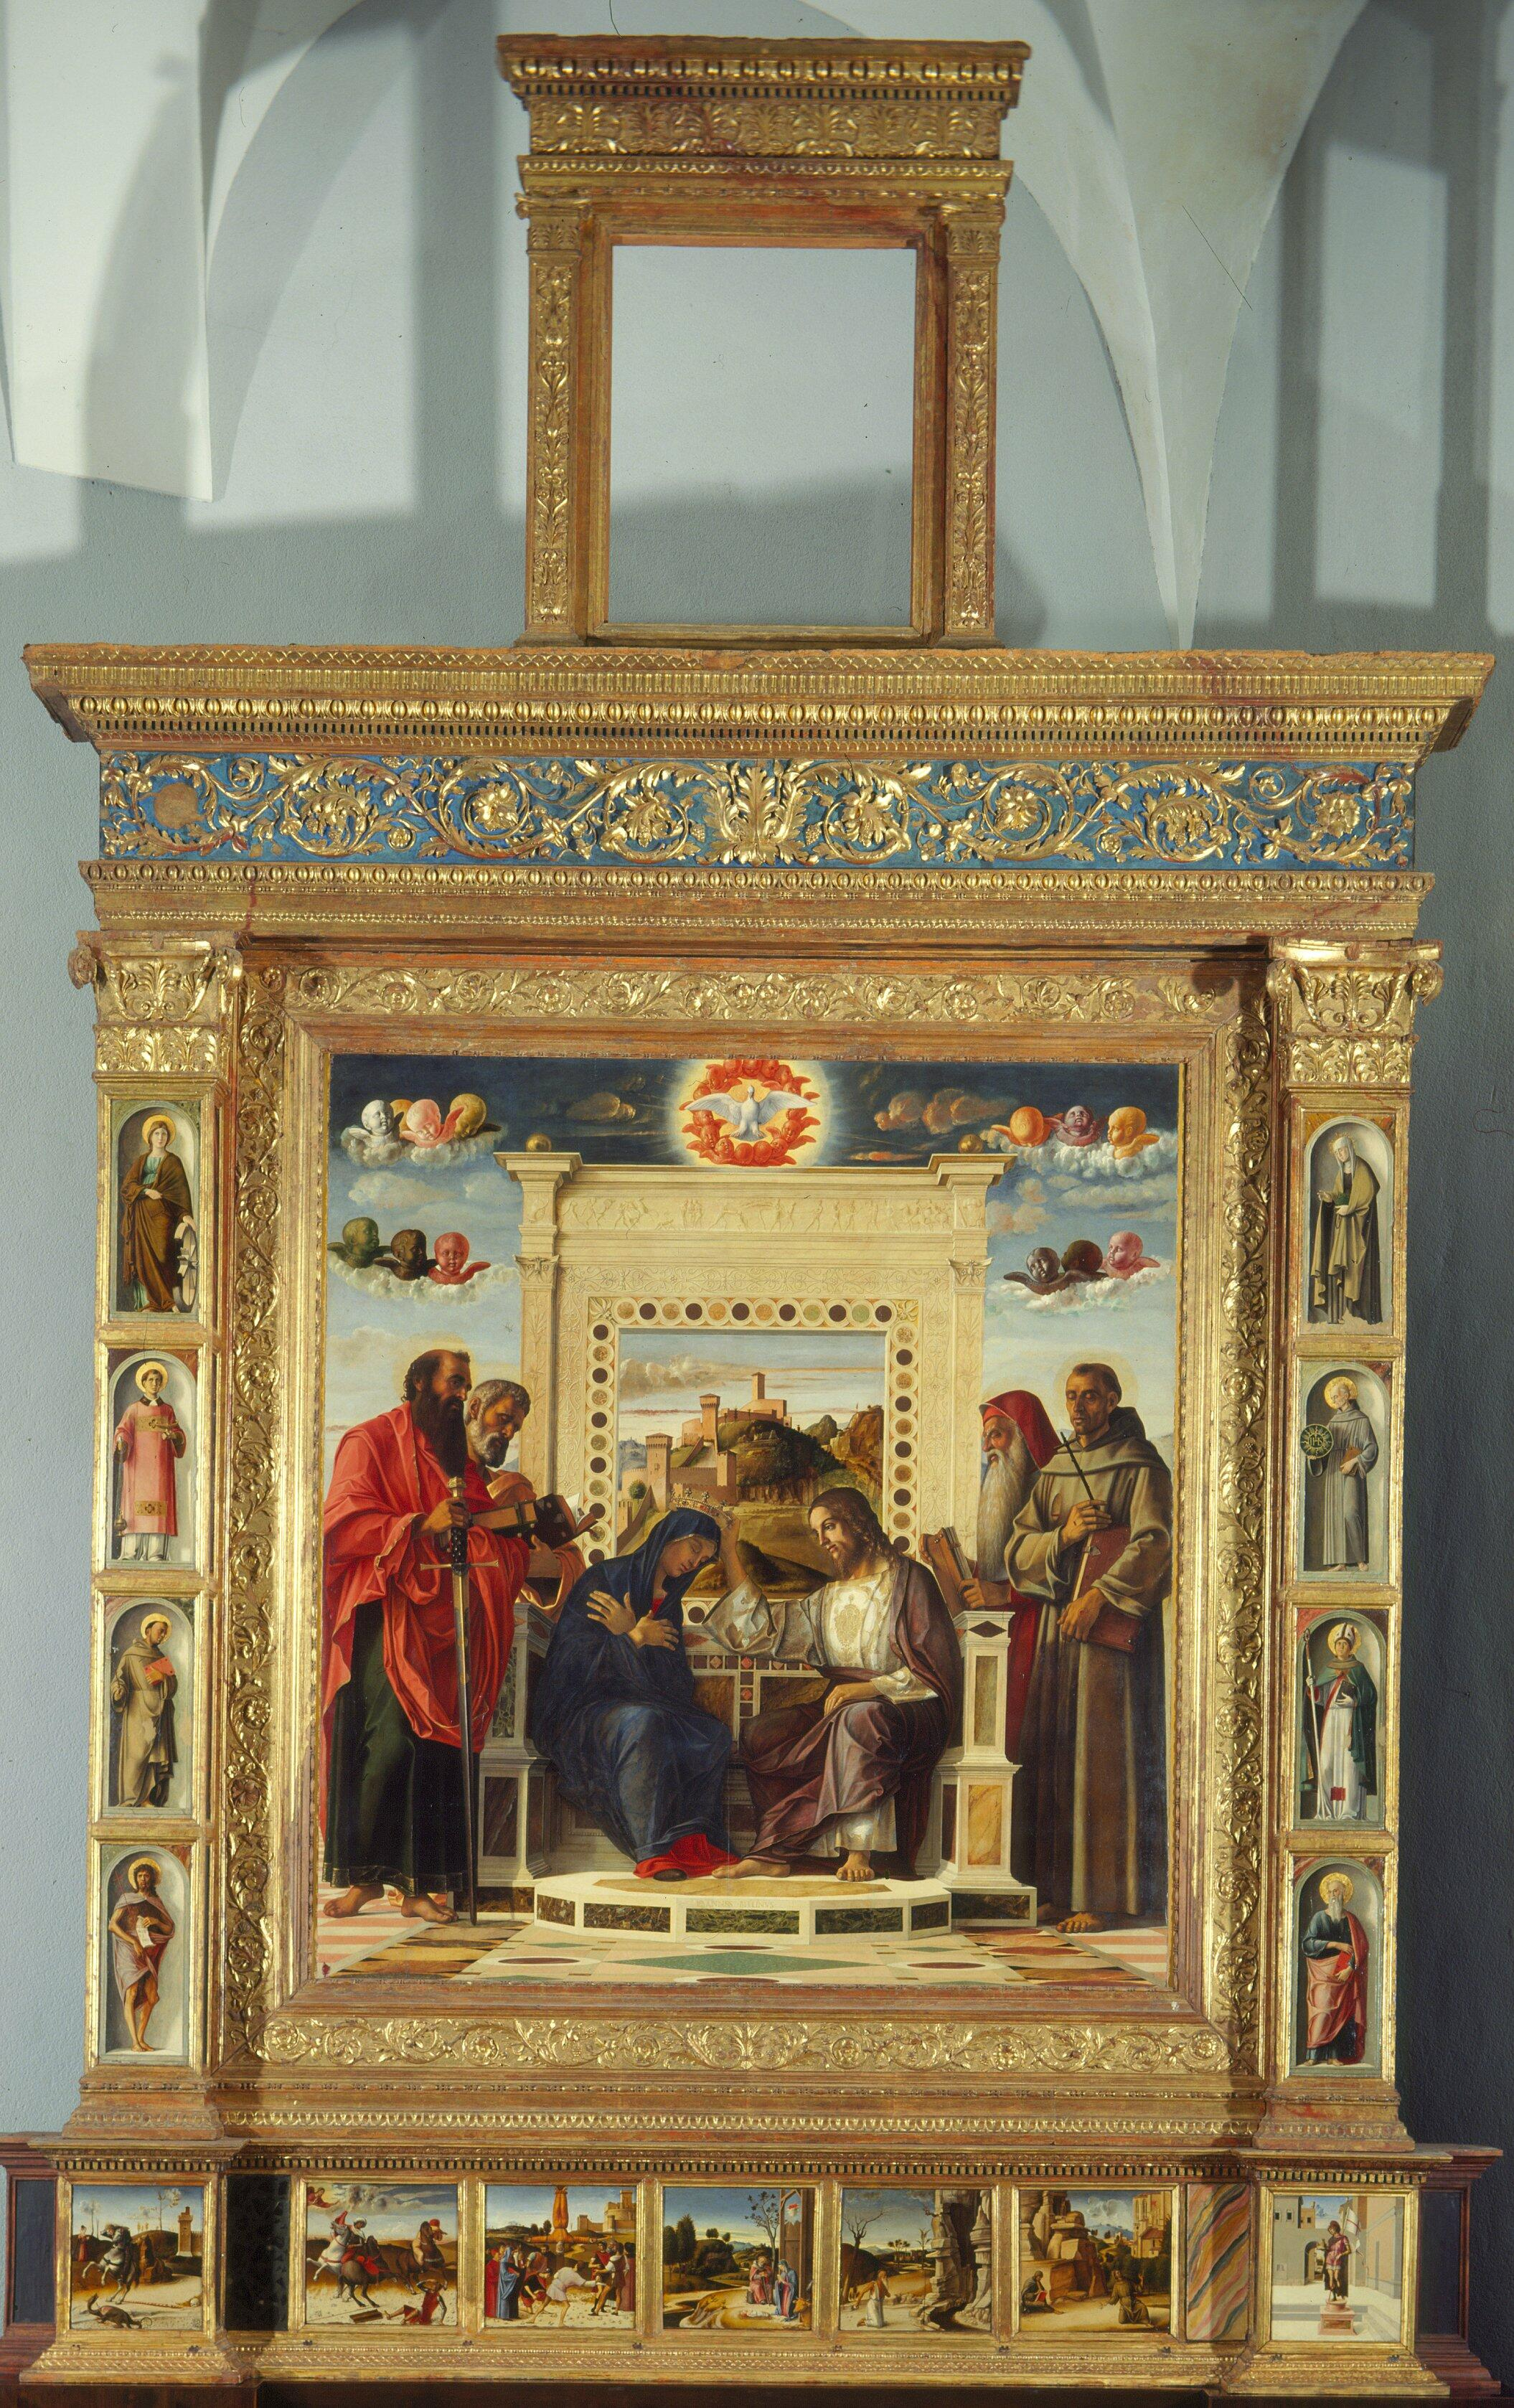
\includegraphics[scale=0.085]{Bellini_Giovanni-Incoronazione_della_Vergine.jpg}}
					\end{center}
					\bigskip
					\begin{center}
					\begin{minipage}{\linewidth}
						\raggedright
						La pala, uno straordinario lavoro di carpenteria, costruito in vista, di un estrema semplicità di montaggio e tenuto insieme mirabilmente da pochi cavicchi di legno, fu dipinta per l'altare maggiore della chiesa di San Francesco a Pesaro.
					\end{minipage}
				\end{center}
			\end{minipage}
		}
	\end{adjustwidth}

	% Background image
	\AddToShipoutPictureBG*{\includegraphics[draft=false, width=\paperwidth,height=\paperheight]{example-image-plain}}
	\newpage
		
	%--------- Page 2 ----------
	
	% First line 
	\begin{tabularx}{\textwidth}{XX}
	{
		\hspace{12mm}
		%Vitale da Bologna - Sant'Ambrogio in trono
		\setdf{content={\textcolor{white}{\hspace{18mm} \Large \#3}}}
		\colorbox{black}{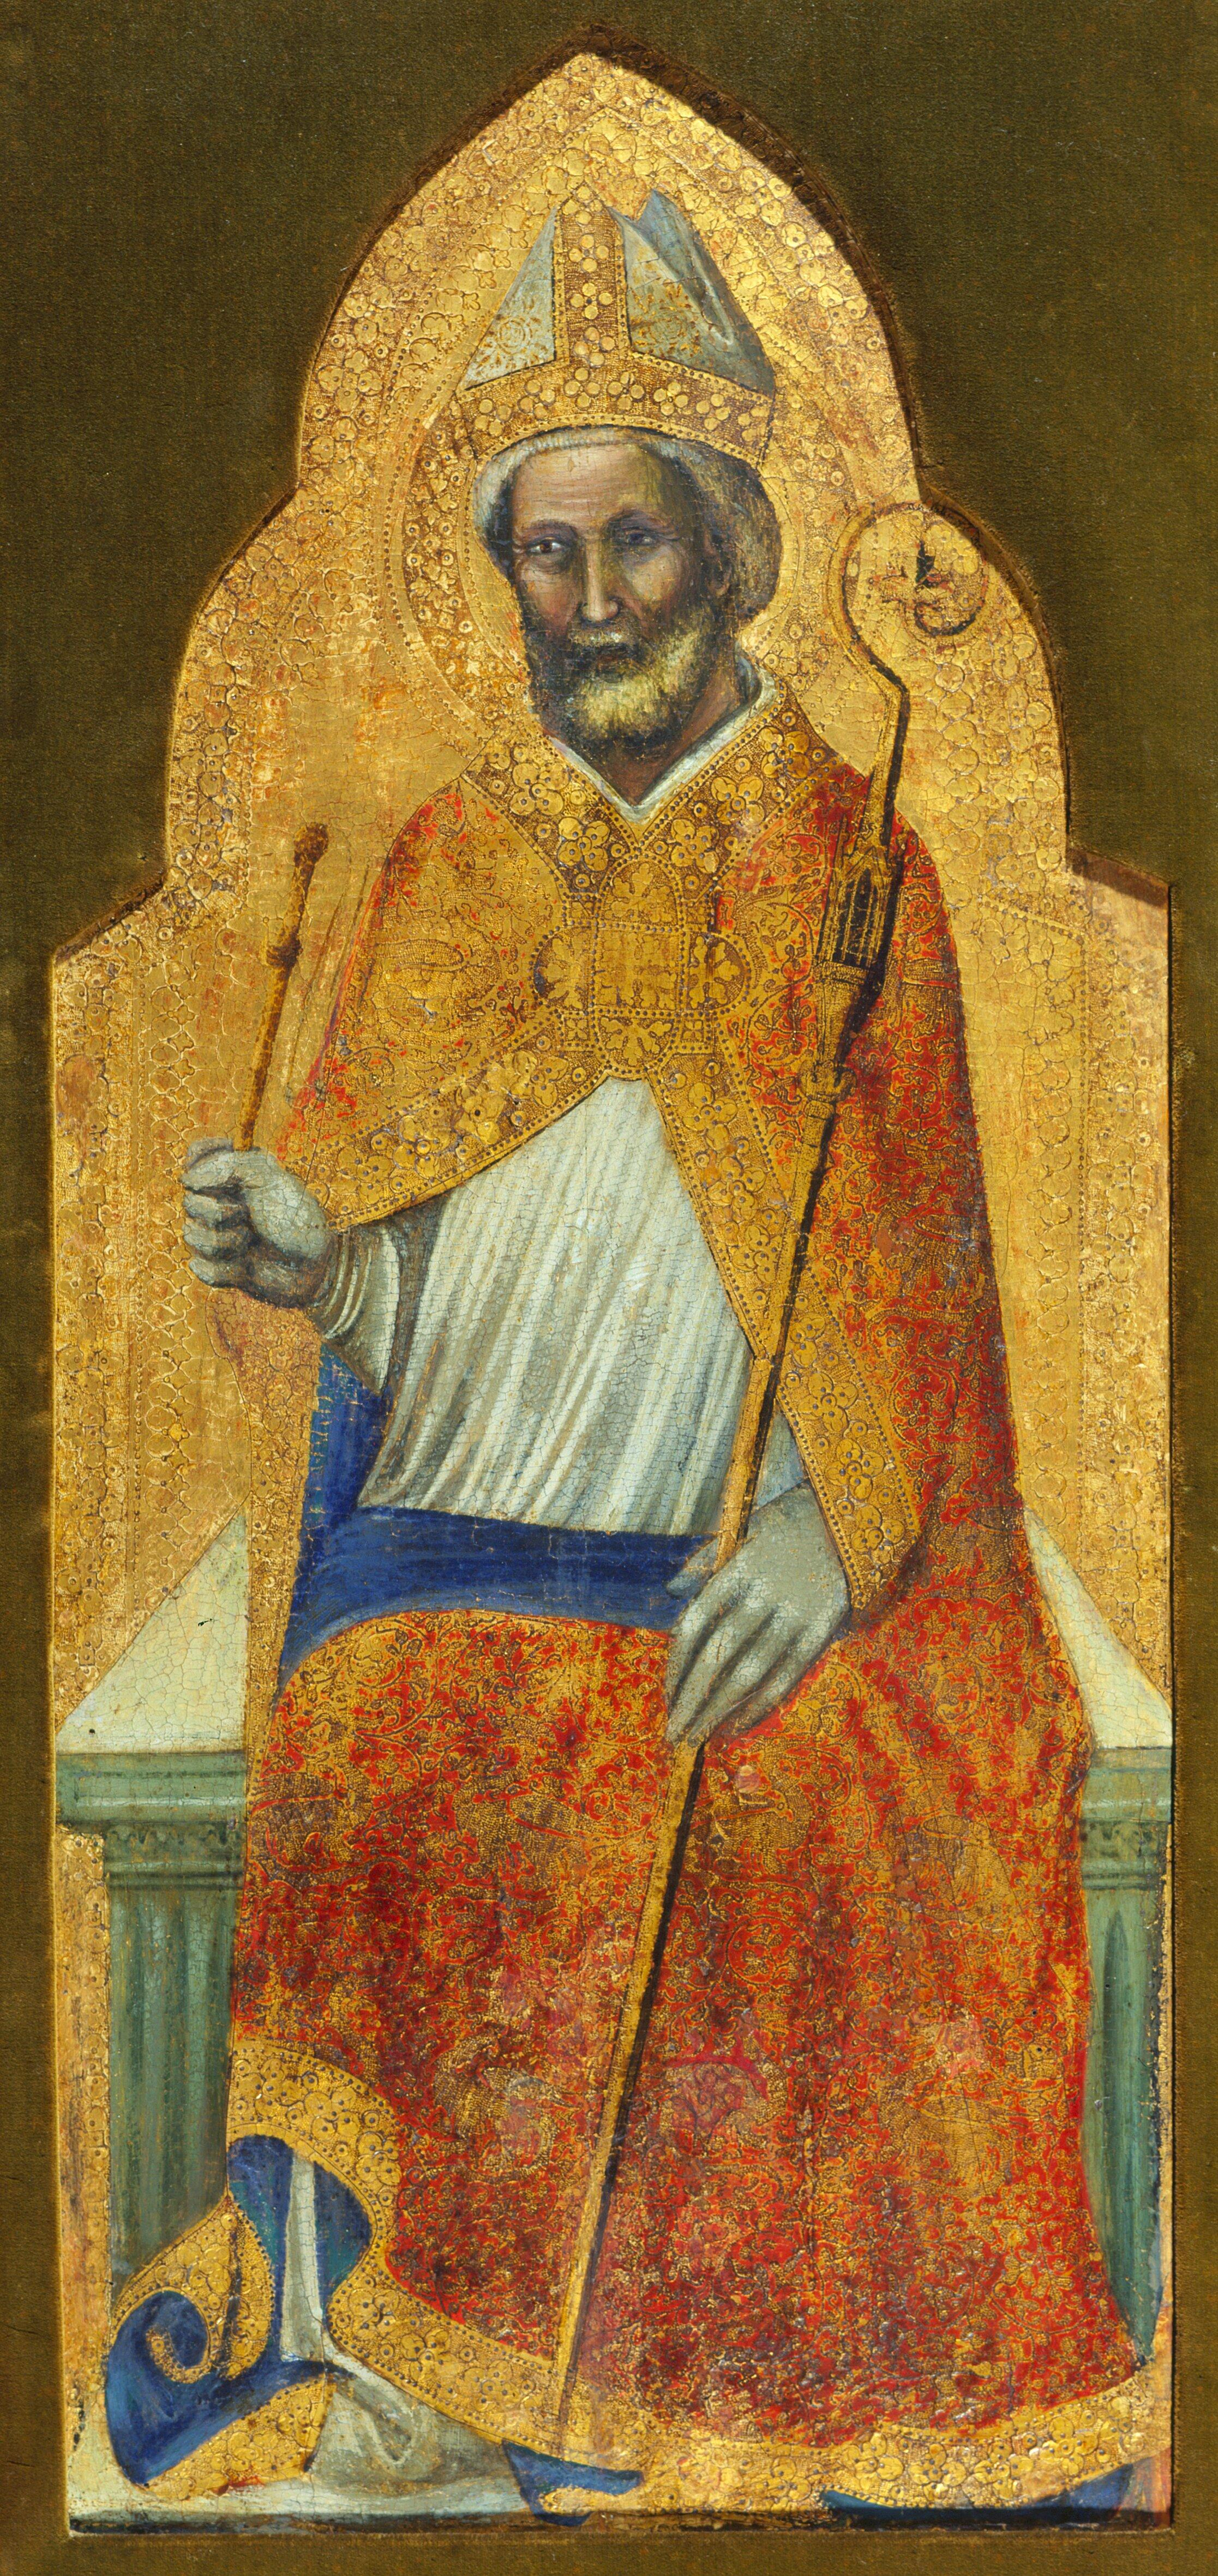
\includegraphics[scale=0.06]{Vitale_da_Bologna-Santo_Ambrogio_in_trono.jpg}}
		\bigskip
		\newline
		\begin{minipage}{0.8\linewidth}
			\raggedright
			Nonostante sia stata sottoposta in tempi recenti a restauro, la tavola presenta ancora nella superficie pittorica varie abrasioni, dovute forse ad antichi restauri, che ne compromettono in parte la leggibilità. Ciò è evidente soprattutto nella zona del viso del santo, fortemente consunta e priva ormai, nella resa dell'incarnato, di quelle connotazioni più morbidamente sfumate che sono tipiche dell'arte vitalesca.
			
		\end{minipage}
		
	}&{
			\hspace{1.5mm}
			% Desani Pietro - Rebecca ed Eleazar
			\setdf{content={\textcolor{white}{\hspace{35mm} \Large \#4}}}
			\colorbox{black}{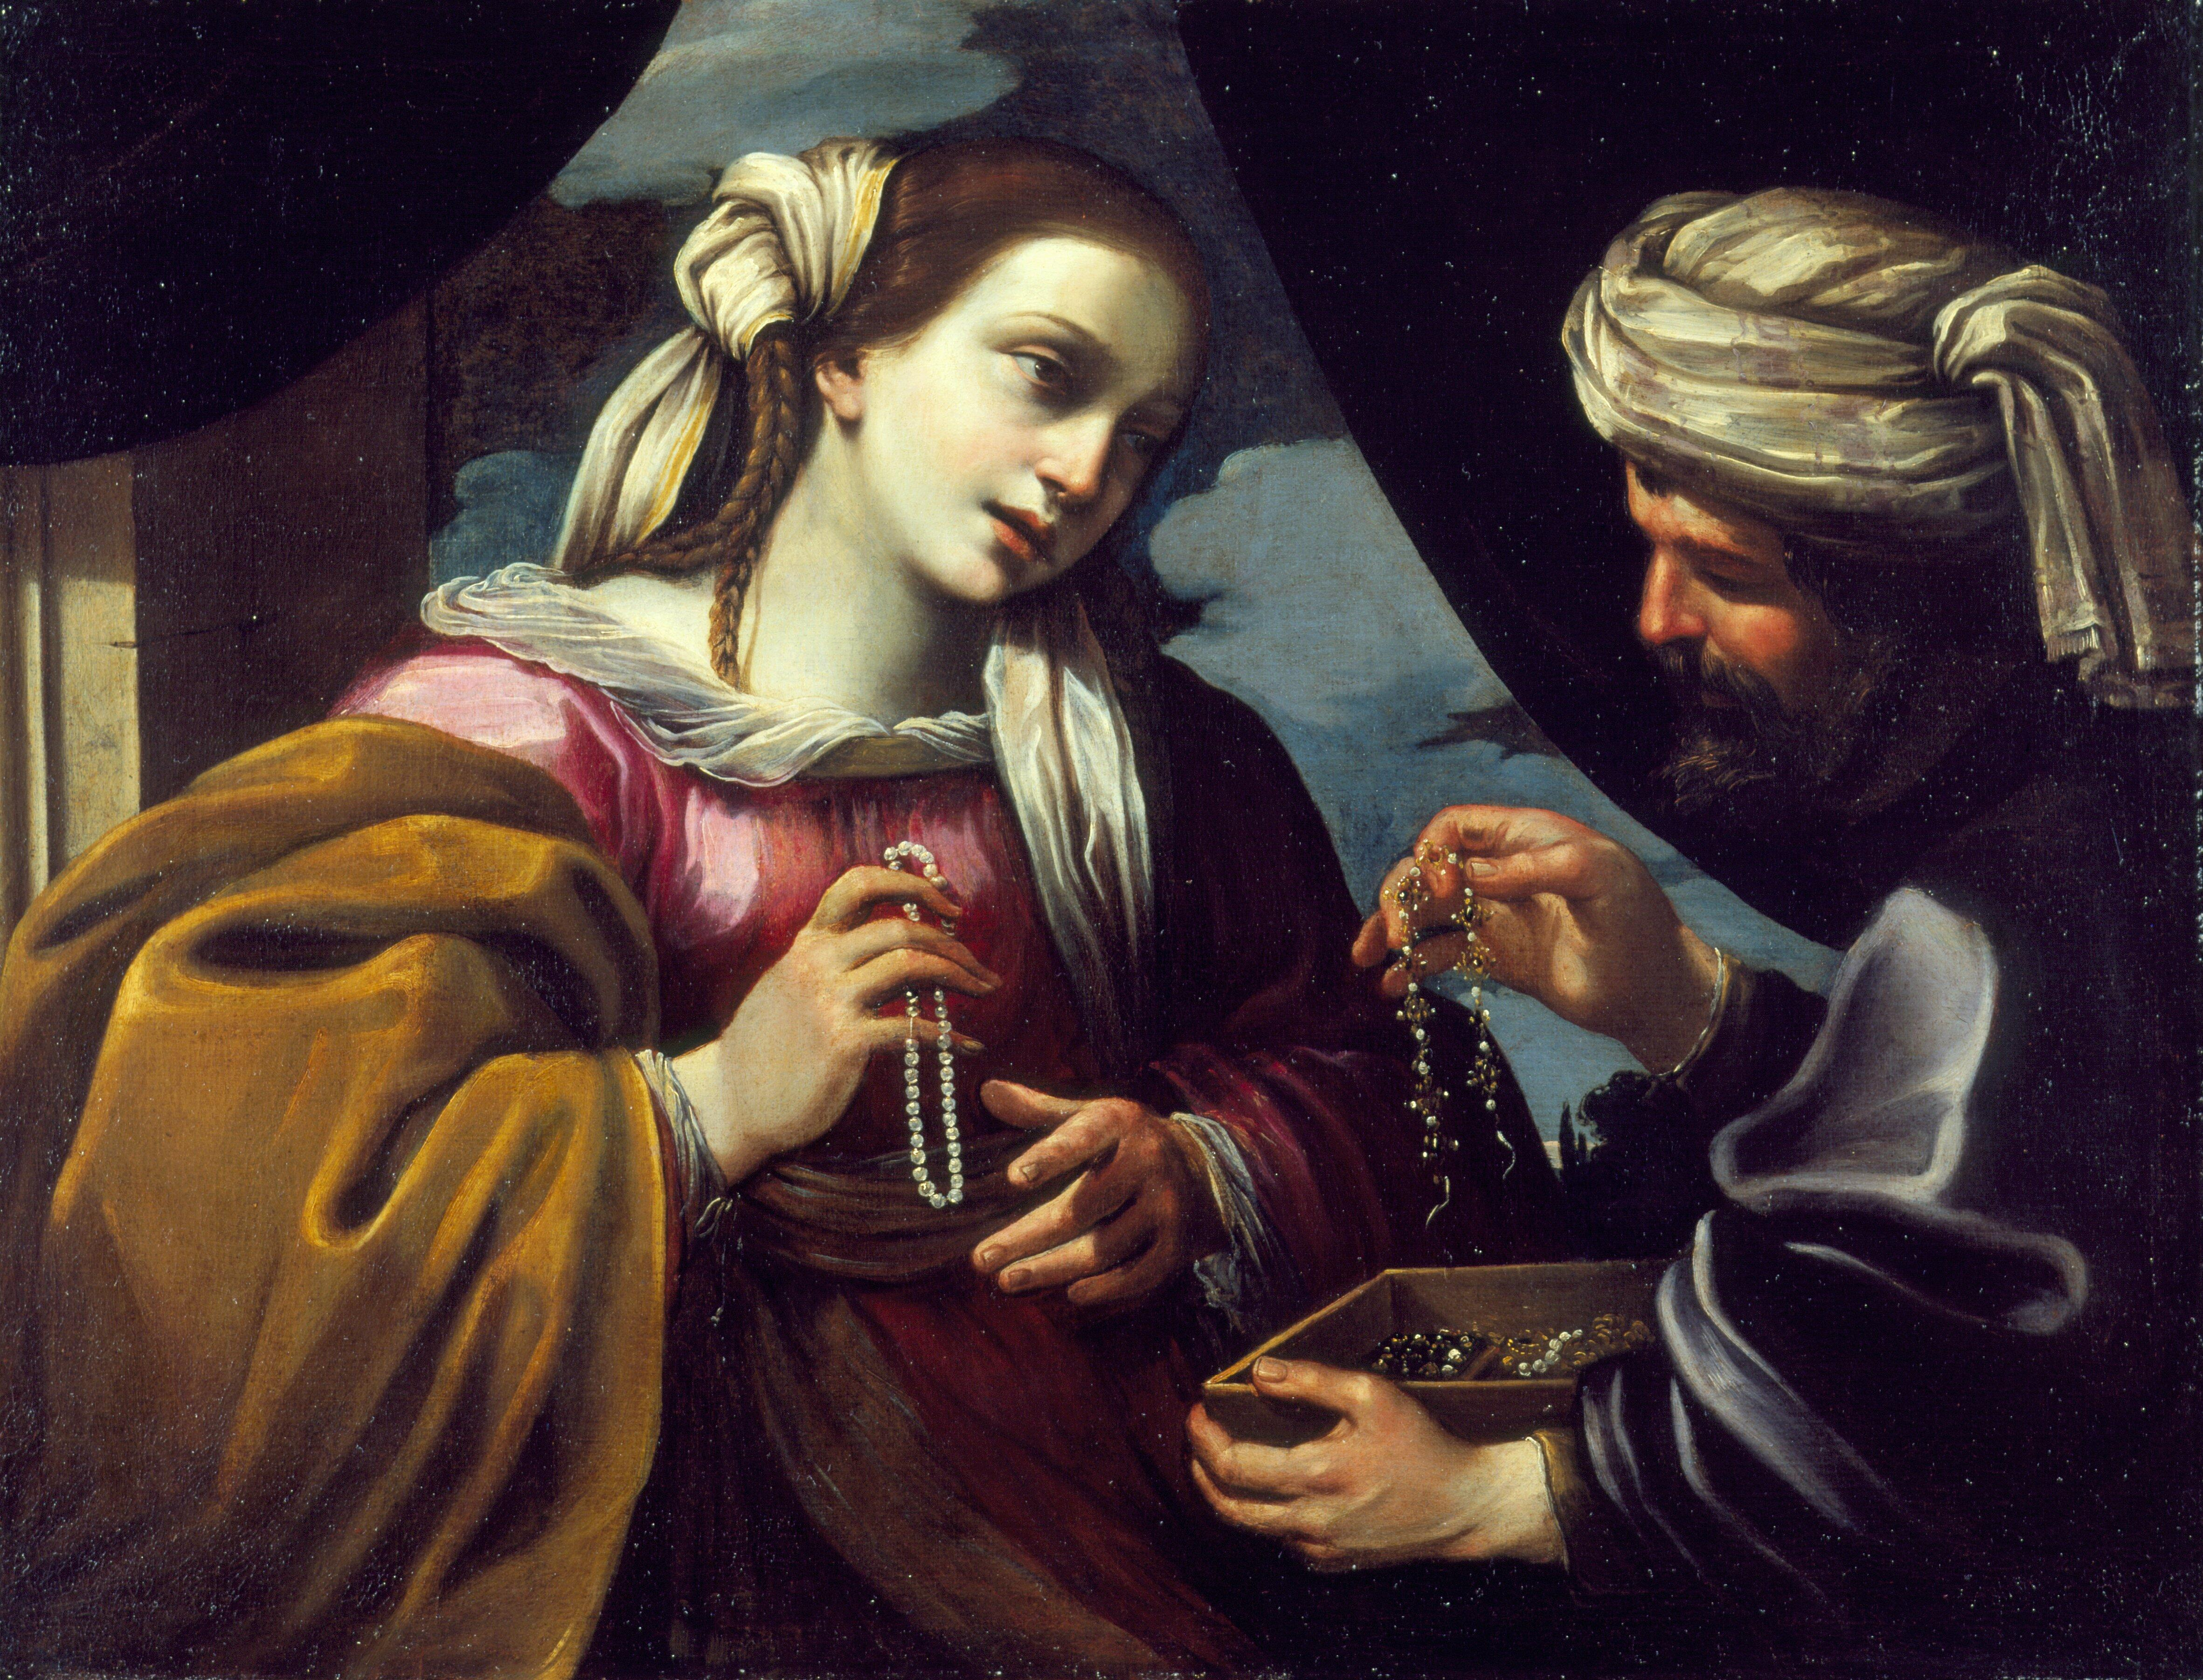
\includegraphics[scale = 0.05]{Desani_Pietro-Rebecca_ed_Eleazar.jpg}}
			\bigskip
			\newline
			\begin{minipage}{0.9\linewidth}
				\raggedright
				Il fido Eleazar, mandato in Mesopotamia da Abramo per cercare una sposa per suo figlio Isacco incontra a un pozzo una fanciulla che lo disseta e alla quale consegna i gioielli che gli sono stati dati per l'eletta.\\
				Secondo quanto si apprende dalle ricerche condotte in questa occasione da Barbara Ghelfi, il dipinto venne ereditato nel 1806 da Maria Malvezzi: nell'occasione veniva detto "Due mezze figure che contrattano delle gioie, d´uno stile che somiglia il Tiarini".
			\end{minipage} 
		}
	\end{tabularx}

	% Second line
	\nopagebreak
	\begin{tabularx}{\textwidth}{X}
	{	
		\begin{center}
			\hspace{27mm}
			%Giovanni Antonio Garella - Leda e il cigno
			\setdf{content={\textcolor{white}{\hspace{20mm} \Large \#5}}}
			\colorbox{black}{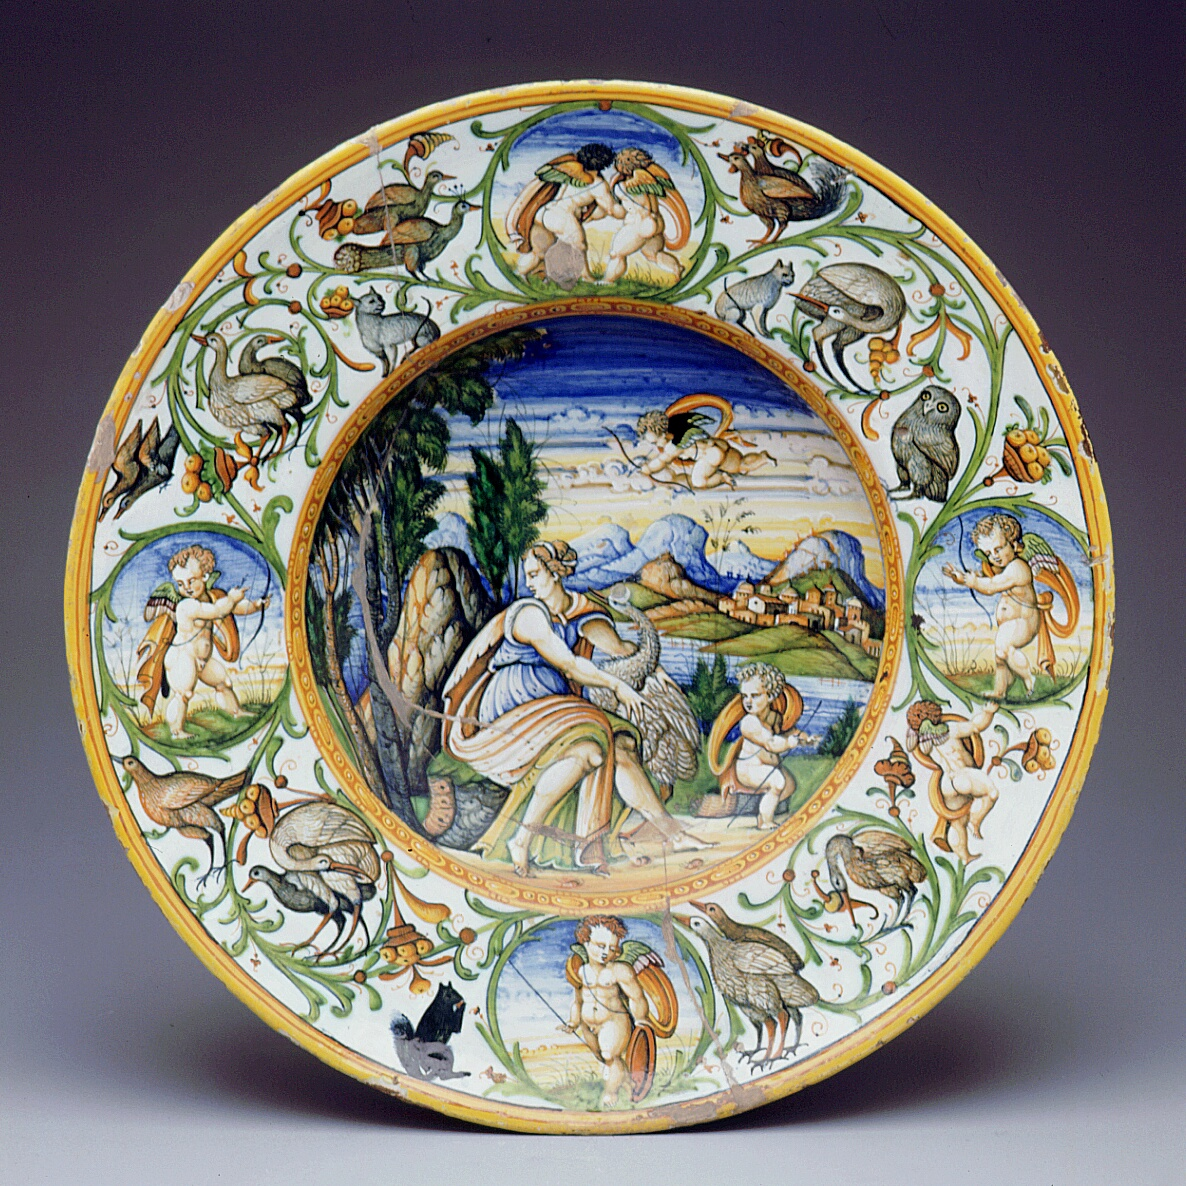
\includegraphics[]{Giovanni_Antonio_Garella-Leda_e_il_cigno.jpg}}
			\bigskip
			\newline
			\begin{minipage}{0.9\linewidth}
					\raggedright
					Il pezzo va riferito senza dubbio alcuno al "Maestro della Conversione di San Paolo": appartengono alla sua mano i caratteri del paesaggio e delle figure, come per esempio il profilo di Leda, che richiama con puntualità quelli degli dipinti sulla tesa.\\
					Ci troviamo di fronte ad un maestro particolarmente capace sia nell'esecuzione delle scene istoriate, sia nella creazione delle raffaellesche, queste ultime eseguite con grande inventiva di dettagli e con mano sicura, molto distanti anche nella tipologia da quelle dei Fontana oppure dei Patanazzi.
			\end{minipage}
		\end{center}
	}
	\end{tabularx}
	
	% Background image
	\AddToShipoutPictureBG*{\includegraphics[draft=false, width=\paperwidth,height=\paperheight]{example-image-plain}}
	\newpage
	
	%--------- Page 3 ----------
	
	% First line 
	\vspace*{\fill}
	\begin{tabularx}{\textwidth}{XX}
		{
			\begin{center}
				\hspace{10mm}
				%Specchio in vetro di Murano
				\setdf{content={\textcolor{white}{\hspace{25mm} \Large \#6}}}
				\colorbox{black}{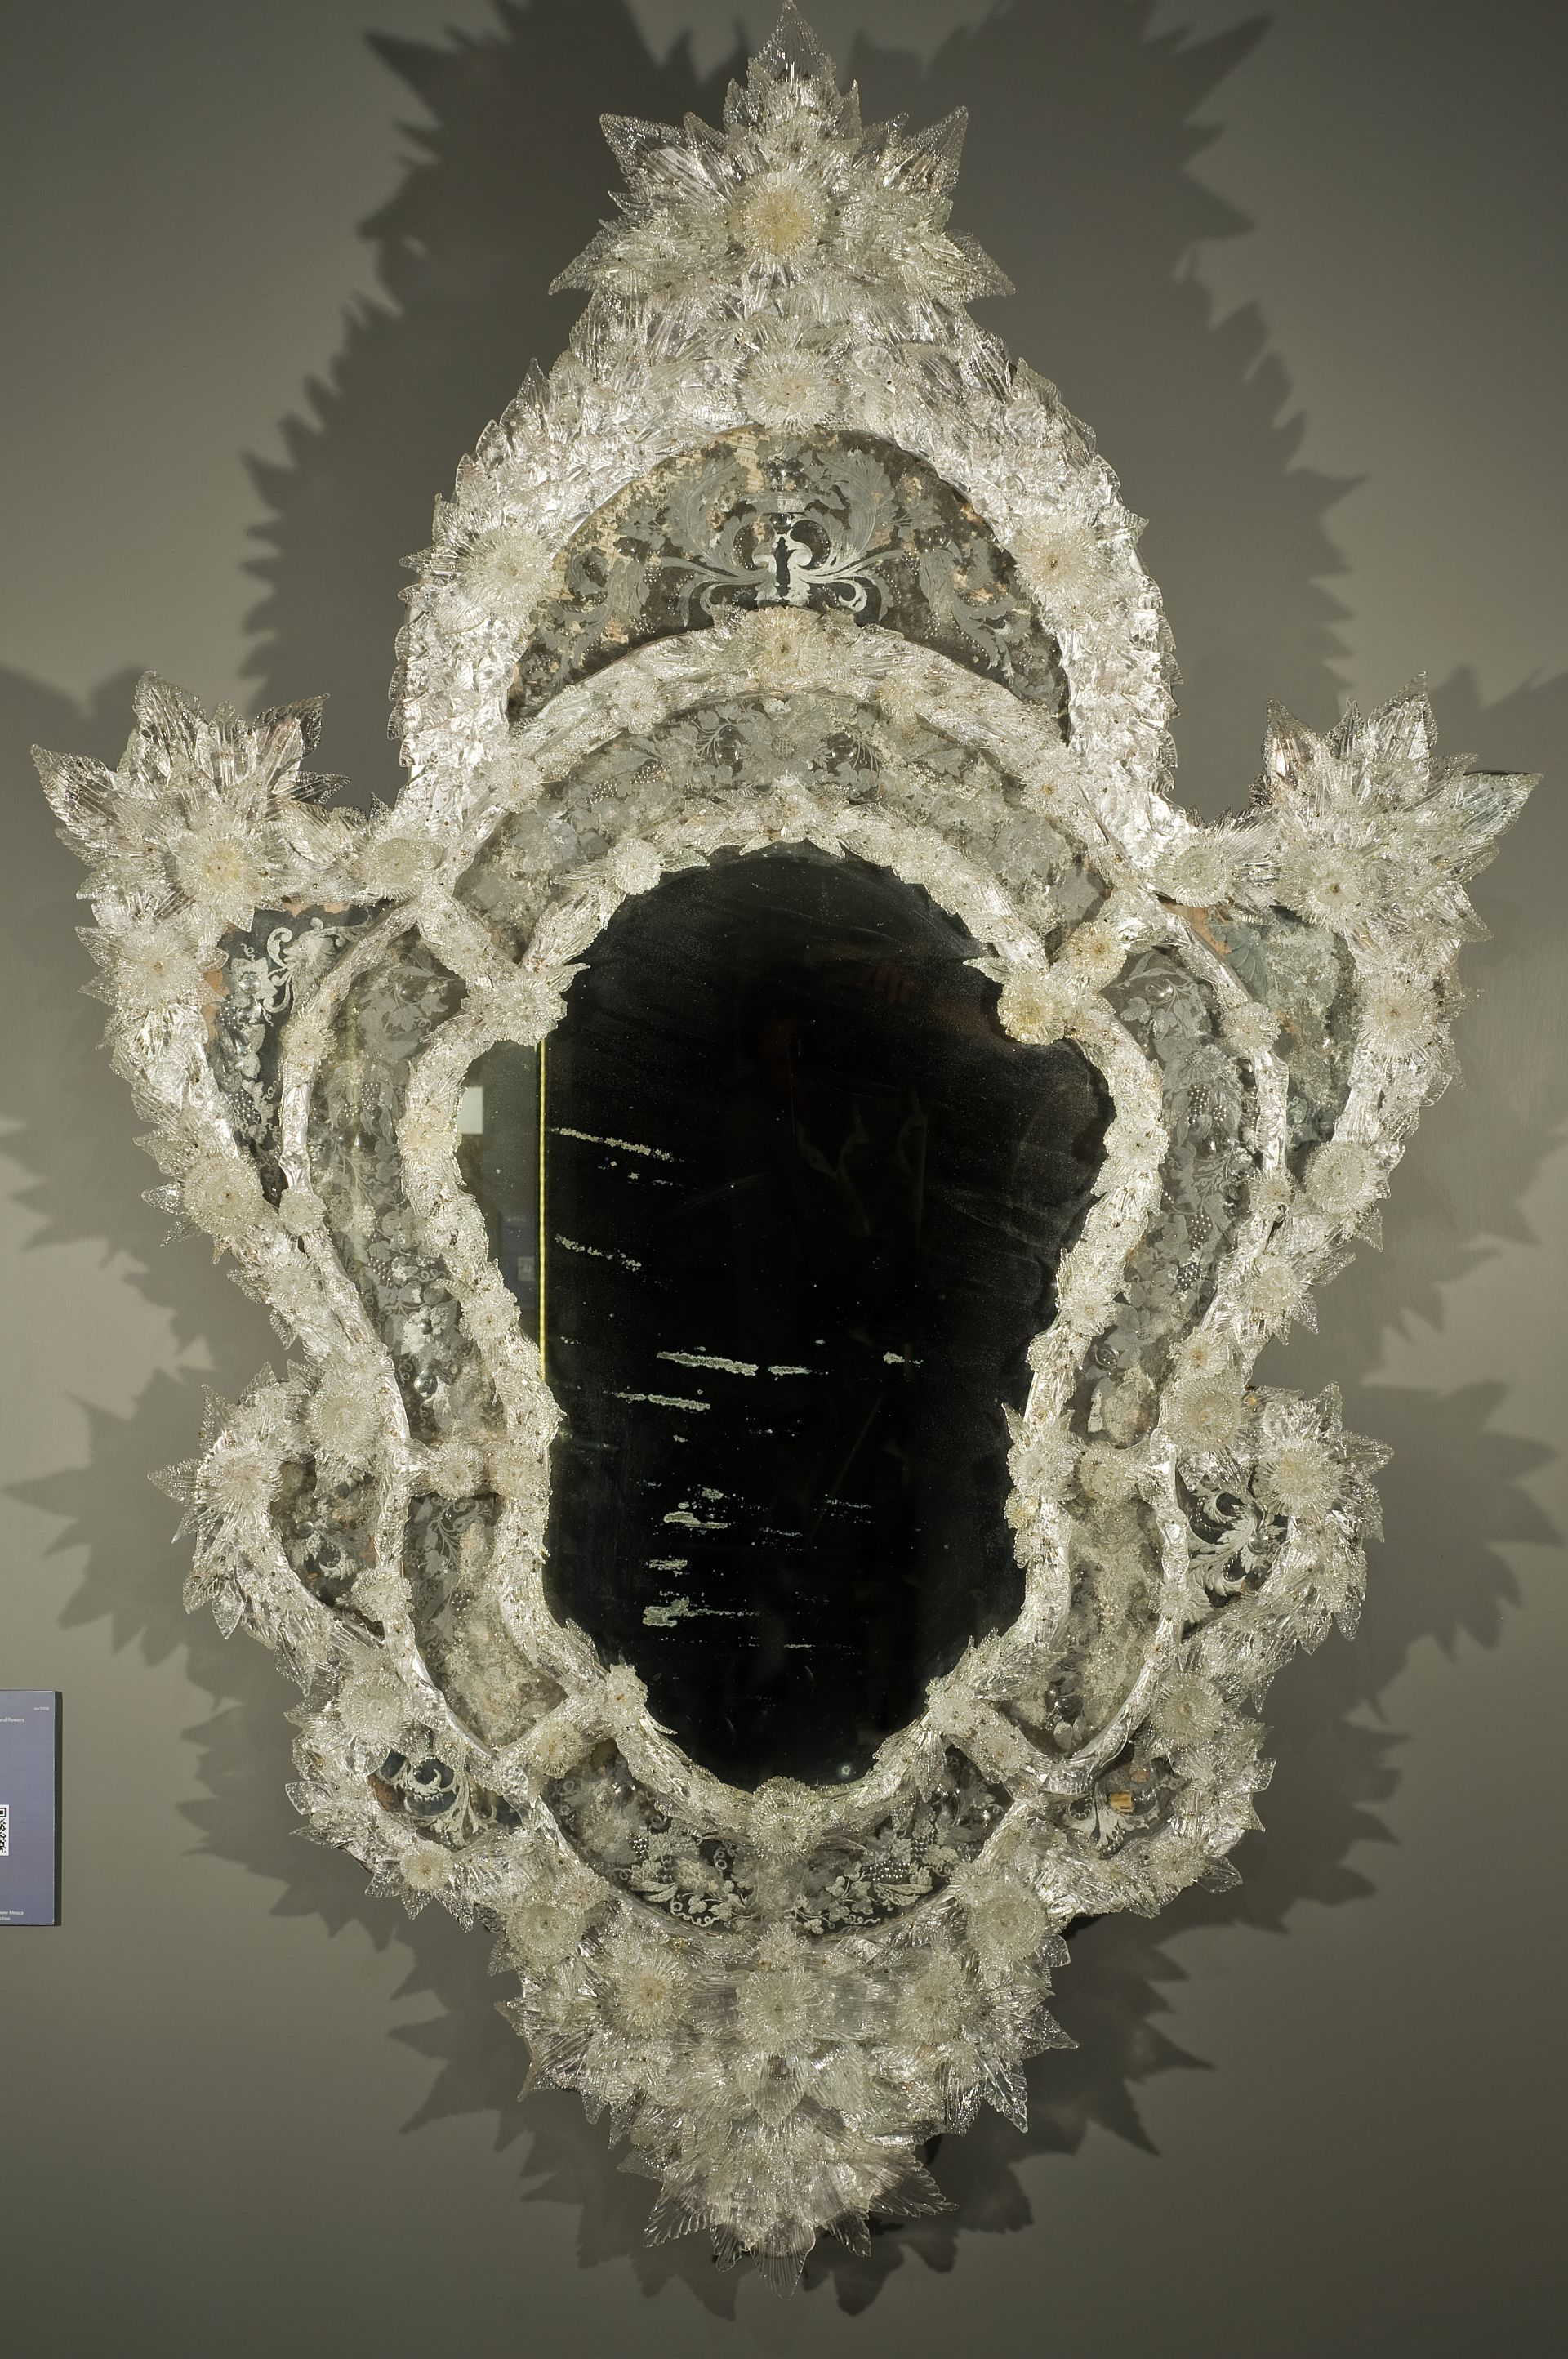
\includegraphics[scale=0.3]{Specchio_di_Murano.jpg}}
				\bigskip
				\newline
				\begin{minipage}{0.8\linewidth}
					\raggedright
					L'opera è una specchiera, si definiscono infatti così gli specchi con cornice fatti per essere appesi alle pareti a scopi funzionali e decorativi.\\ 
					Realizzata tra la fine del Settecento e l'inizio dell'Ottocento, è decorata con foglie e fiori in vetro che costituiscono la  peculiarità delle specchiere artistiche di Murano.\\
					La produzione muranese nel Settecento eleva il livello medio della produzione ad un grado di eleganza e raffinatezza mai raggiunto prima.
				\end{minipage}
			\end{center}
			
		}&{
			\vspace{20mm}
				%Vedute di Roma
				\hspace{10mm}{
				\setdf{content={\textcolor{white}{\hspace{30mm} \Large \#7}}}
				\colorbox{black}{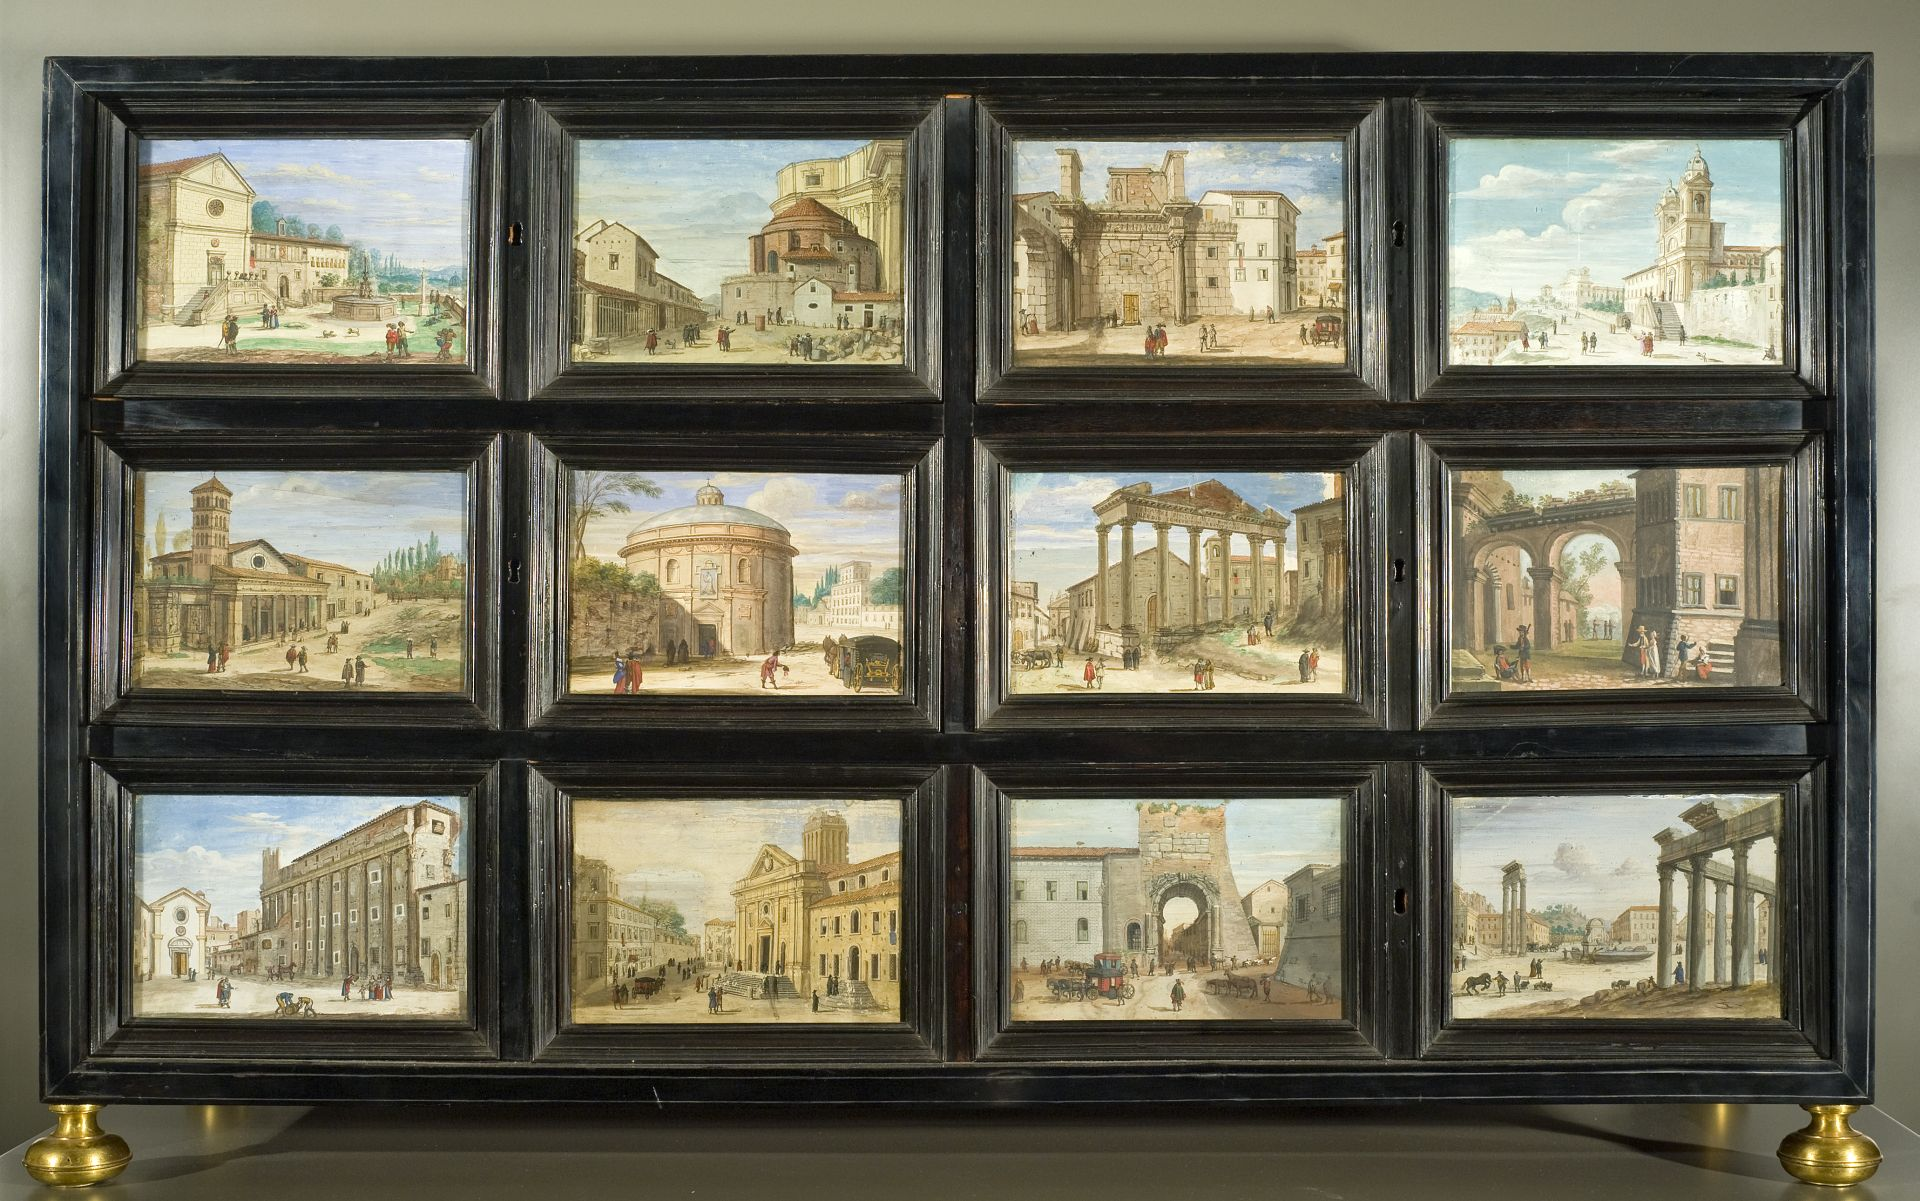
\includegraphics[scale=0.35]{Vedute_di_Roma_1.jpg}}
				}
				%\bigskip
				%\newline
				\begin{center}
					\begin{minipage}{0.7\linewidth}
						\raggedright
						L'usanza di decorare il fronte di stipi e studioli con placche raffiguranti vedute dell'urbe deve essere fatta risalire agli anni Sessanta del Seicento, come si può vedere nella parte interna dello stipo eseguito dall'ebanista Giacomo Herman nel 1668 e attualmente al Kunsthistorisches Museum di Vienna. Va inoltre notato che il tipo di veduta che tende a riprodurre in maniera pressoché fedele il luogo rappresentato si afferma a Roma attorno agli anni Trenta del Seicento, con la presenza a Roma del pittore strasburghese Willhelm Baur.
					\end{minipage}
				\end{center}
		}
	\end{tabularx}
	\vspace*{\fill}
	
	% Background image
	\AddToShipoutPictureBG*{\includegraphics[draft=false, width=\paperwidth,height=\paperheight]{example-image-plain}}
	\newpage
	
\end{document}